\hypertarget{section-concepts}{%
\section{Crosscutting Concepts and Architectural Decisions}\label{section-concepts}}

\textbf{Content}

This section describes overall, principal regulations and solution ideas that are relevant in multiple parts (= crosscutting) of our system and its architecture. Such concepts and decisions are often related to multiple building blocks and can include many different topics, such as

\begin{itemize}
  \item
    models, especially domain models
  \item
    architecture or design patterns
  \item
    rules for using specific technology
  \item
    principal, often technical decisions of an overarching nature
  \item
    implementation rules
  \end{itemize}

\subsection{Frontend}

\subsubsection{Domain Model \& Data Structures}
The Vivendo Webshop frontend relies on several key data models that keep information consistent across different parts of the application:

\begin{itemize}
  \item \textbf{Product Model}: This structure includes fields such as the product ID, name, description, price, and stock level. Any part of the webshop that displays or updates product information---including the Shop Module and the Admin Dashboard---uses this same model.
  
  \item \textbf{Cart Item Model}: This extends the Product Model by incorporating cart-related details, such as quantity or item-level notes. The Cart Context employs this structure to ensure that updates to product attributes, like pricing or availability, remain in sync with a user's cart.
  
  \item \textbf{Message Model}: This standardized format describes user inquiries with fields such as subject, sender information, and message text. Both the Contact Module and the Admin Dashboard interact with this single model to create, display, and manage messages consistently.
\end{itemize}

We maintain these data models as shared sources of truth (SSOT). Splitting them into different product models for the shop and the admin area would risk creating mismatches if one model would be updated without the other. It would also complicate maintenance, since any field changes would need to be replicated in multiple places. By using these core structures throughout the system, we reduce the likelihood of data inconsistencies and simplify ongoing feature development.

\subsubsection{UI \& UX Conventions}
All pages in the Vivendo Webshop share a unified layout and design language. A global layout component (\texttt{layout.jsx}) includes site-wide elements such as the header, footer and navigation links. This approach guarantees that the user experience remains consistent across all modules. Tailwind CSS is used to provide a utility-first styling approach so that developers can quickly apply spacing, color, and typography classes to maintain uniform visuals. 

We selected Tailwind because of its flexibility and the minimal overhead it adds, Although other frameworks like Bootstrap might provide predefined components, those often require extensive overrides to achieve a specific kind of identity. 

\subsubsection{Routing \& Folder Structure (Next.js)}
Our Next.js setup uses file-based routing to map files within the \texttt{pages/} directory to distinct routes. This arrangement makes the URL structure predictable for both developers and users. Public pages - including the shop, cart, and contact form - reside under straightforward displayed paths, while administrative features such as login or the Admin Dashboard are kept separate to detach sensitive functionality.

We chose Next.js because it offers server-side rendering and built-in image optimization. These features are valuable for an online shop (e.g. Vivendo) where both SEO and performance are important. Besides alternative solutions, Next.js fits best with the platform's requirement for dynamic content, simple configuration and a strong user experience across devices.

\subsubsection{Shared State Management}
React Context API is used to share and manage global data. For example, the Cart Context holds a user’s cart items and provides methods to add, remove, or update them. By centralizing cart logic, all components in the webshop - from product pages to checkout flows - operate on the same state and can render consistent information. 

\subsubsection{Security \& Authentication}
The webshop uses an authentication-based route for the dashboard including all administrative features. This ensures that unauthorized individuals cannot edit products or read messages. The current approach checks whether the username and password match the required values and if valid, stores them in a local storage to simulate a logged-in state. This design is sufficient for a simple prototype but would need to be replaced with a more secure solution in a production environment.

For payment processing the system depends on Stripe to handle sensitive credit card data. This reliance on a secure external provider reduces compliance overhead for our team and limits the exposure of critical payment details in our infrastructure. We selected Stripe based on its popularity, strong security posture and clear documentation for the integration with Next.js. 

\subsubsection{Error Handling \& Logging}
React error boundaries catch unexpected exceptions in key components, preventing the entire application from failing if one feature encounters a problem. 

\subsubsection{Consolidated Architectural Decisions}
\begin{itemize}
  \item \textbf{Next.js} is our framework for delivering server-rendered pages and handling routing automatically.
  \item \textbf{Stripe} is used for payment processing, removing the need to manage credit card data in our own systems.
  \item \textbf{React Context} manages global state, such as the shopping cart, in order to reduce boilerplate and maintain clarity.
  \item \textbf{Single Source of Truth} for data models avoids the duplication of field definitions across modules.
\end{itemize}

These decisions ensure that the our frontend remains flexible and performant through maintaining an architecture that is adaptable as the platform evolves.

\subsection{Backend}
\subsubsection{Domain Model \& Data Structures}

\begin{figure}[h]
    \centering
    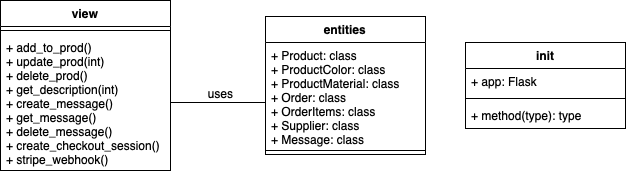
\includegraphics[width=0.9\textwidth]{images/uml_backend.png}
    \caption{Backend Domain Model}
    \label{fig:doman-model-backend}
\end{figure}

Figure \ref{fig:doman-model-backend} illustrates the main structure of the backend. As discussed in Section \ref{section-solution-strategy}, the backend is designed to be lightweight, with no specific design pattern applied. There is an association between the view and entity layers, as the view script interacts with the entity classes when saving data to the database.

The init script, as the name suggests, initializes the app variable, which is required throughout other scripts in the backend.

The entities script defines classes that represent the database tables. These data structures are then utilized within the views script to perform CRUD operations.

\begin{figure}[h]
    \centering
    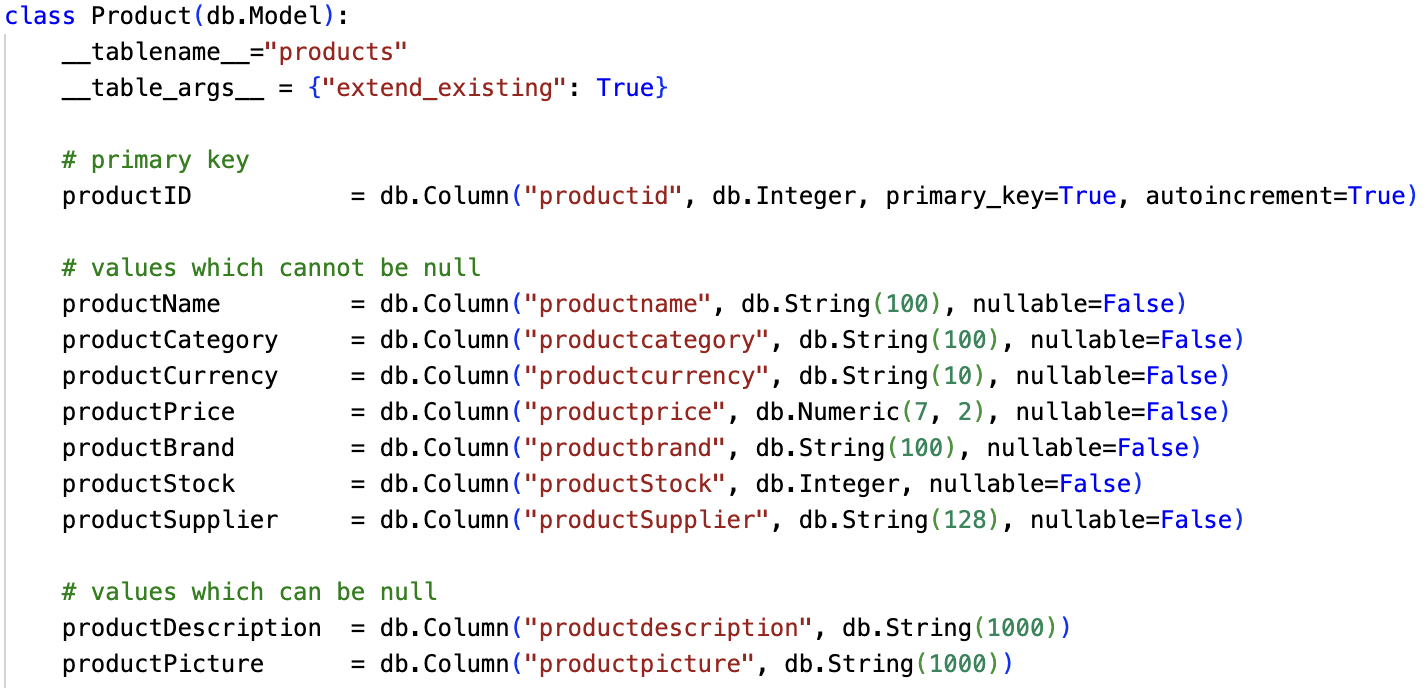
\includegraphics[width=\textwidth]{images/code_entity_example.png}
    \caption{Structure of Product Entity}
    \label{fig:db-entity}
\end{figure}

Figure \ref{fig:db-entity} displays the entity object representing the Product table. This data structure allows us to store and manage the various products offered by the Vivendo webshop. Similar entity objects are used for all tables in the database to ensure consistent handling of data.

\subsubsection{User Experience Concept}
While the backend does not directly influence the look and feel of the user interface, it plays an important role in enhancing the overall user experience by providing clear and informative push notifications. These messages notify users when an action is successful or unsuccessful, helping to keep them informed throughout their interaction with the system.

Additionally, the frontend interacts with the backend through RESTful API endpoints, allowing users to retrieve data in JSON format. This seamless integration between frontend and backend ensures that data is delivered efficiently and consistently to improve the user experience.

\subsubsection{Implementation rules}
\textbf{JSON Validation Concept} \\
In the views script, each endpoint begins by checking whether the incoming request object is in JSON format. This serves two main purposes: first, it ensures that the data follows the agreed-upon format; second, it simplifies data handling for the backend developer. Once the data format is verified, the appropriate actions are taken based on the type of operation.

\textbf{Single Responsibility Concept} \\
Another key principle followed in the backend was ensuring that each function performs only one operation at a time. Although Flask allows handling multiple CRUD operations within a single function by specifying them in the route decorator and filtering requests using if-statements, this approach was avoided. Instead, each CRUD operation was assigned its own function to maintain a clear and organized backend code structure.

\textbf{Response Messaging Concept} \\
Thirdly, if any exception occurs during the processing of the request data, either an HTTP 400 error (for bad requests) or an HTTP 500 error (for internal server issues) is returned to the frontend, along with a detailed message. This message is used to inform the user that an issue has occurred and to provide more context, ensuring they are aware that something went wrong. In cases where the request is successfully processed, an HTTP 200 status code is returned, accompanied by a message or some data from the database confirming that the operation was completed successfully, tailored to the specific action performed.